\label{sec:pileup}

During the data taking the instantaneous LHC luminosity exceeded
$\approx$ $3.0 \times 10^{33}$ cm$^{-2}$ s$^{-1}$, 
or an average of ten interactions per bunch crossing. 
Such pileup collisions are not correlated with the hard-scattering
 process that triggers an interesting event, but present a background
 from low-$\pt$ interactions that can affect the measured energies of 
jets and their observed masses. 
 Methods to mitigate these effects are part of standard event 
reconstruction, as discussed in Section~\ref{evrecosection}, 
and are essential for extracting correct jet multiplicities and energies.
The jet mass is expected to be particularly sensitive to pileup~\cite{jetsub}
for jets of large angular extent that contain many
particles. Grooming techniques are designed to reduce the effective
area of such jets and thereby minimize sensitivity to pileup. 
We examine this issue through 
%%MC 
studies of jet mass in the presence of pileup. 

The mean jet mass $\langle m_J \rangle$ for AK jets is presented for
size parameters $R = 0.5$, 0.7, and 0.8, as a function of the total number of reconstructed
primary vertices ($N_{\mathrm{PV}}$) in
Fig.~\ref{figs:histAK7MjetVsNvtx_nvtxPlots}(a), for data and MC simulation. 
The mean mass for $N_{\mathrm{PV}}=1$ increases
linearly with the jet radius from 0.5 to 0.8. A measure of the
dependence of $\langle m_J \rangle$ on pileup is given by the slope of a
linear fit to the jet mass versus $N_{\mathrm{PV}}$. The ratios of these 
slopes ($s_R$) are found to be roughly consistent with the ratio of the third
power of the jet radius, as summarized in Table~\ref{tab:slopes}.  

\begin{table}[!h]
\caption{Slopes of linear fits of $\langle m_J \rangle$ as a function
  of $N_{\mathrm{PV}}$ for AK jets of different $R$ values.}
\label{tab:slopes}
\begin{center}
\begin{tabular}{ccc} \hline\hline
Ratio of Slopes & Measured & Expected \\ \hline
\hline\rule{0pt}{12pt}
$s_{0.7}/s_{0.5}$ & $2.7 \pm 0.9~(\rm{stat.})$ & $(0.7/0.5)^3 = 2.74$  \\
$s_{0.8}/s_{0.5}$ & $3.3 \pm 1.0~(\rm{stat.})$ & $(0.8/0.5)^3 = 4.10$  \\
$s_{0.8}/s_{0.7}$ & $1.2 \pm 0.2~(\rm{stat.})$ & $(0.8/0.7)^3 = 1.49$  \\
\hline\hline
\end{tabular}
\end{center}
\end{table}


\noindent This is in agreement with predictions for scaling of the mean mass~\cite{Dasgupta:2008}. The $R^3$ dependence can be understood in terms of the increase of the jet area as $R^2$. Simultaneously, the contribution of these particles to the jet mass scales with the distance between them, or ${\approx} R/2$, yielding another power of $R$.

In Fig.~\ref{figs:histAK7MjetVsNvtx_nvtxPlots}(b) we show the
dependence of $\langle m_J \rangle$ on $N_{\mathrm{PV}}$, for AK7 jets, for
different grooming algorithms. The grooming significantly reduces the
impact of pileup on $\langle m_J \rangle$, as reflected by the decrease
of the slope of the linear fit to the groomed-jet data points, as
summarized in Table~\ref{tab:slopes2}.

  
%In Figure~\ref{figs:histAK7MjetVsNvtx_nvtxPlots2} we show the ratio of the groomed and ungroomed jet mass as a function of $N_{\mathrm{PV}}$. It can be observed that the two most aggressive grooming algorithms do not have a strong dependence on PU, while the least aggressive filtering algorithm becomes more effective in reducing the ungroomed jet mass for high PU. As also shown in Fig.~\ref{figs:histAK7PtAvgVsMjetGroomOverReco_ratioPlots}, the grooming in the simulation overestimates the jet mass reduction for the trimming and pruning algorithms. 

\begin{figure}[htbp]
\centering
%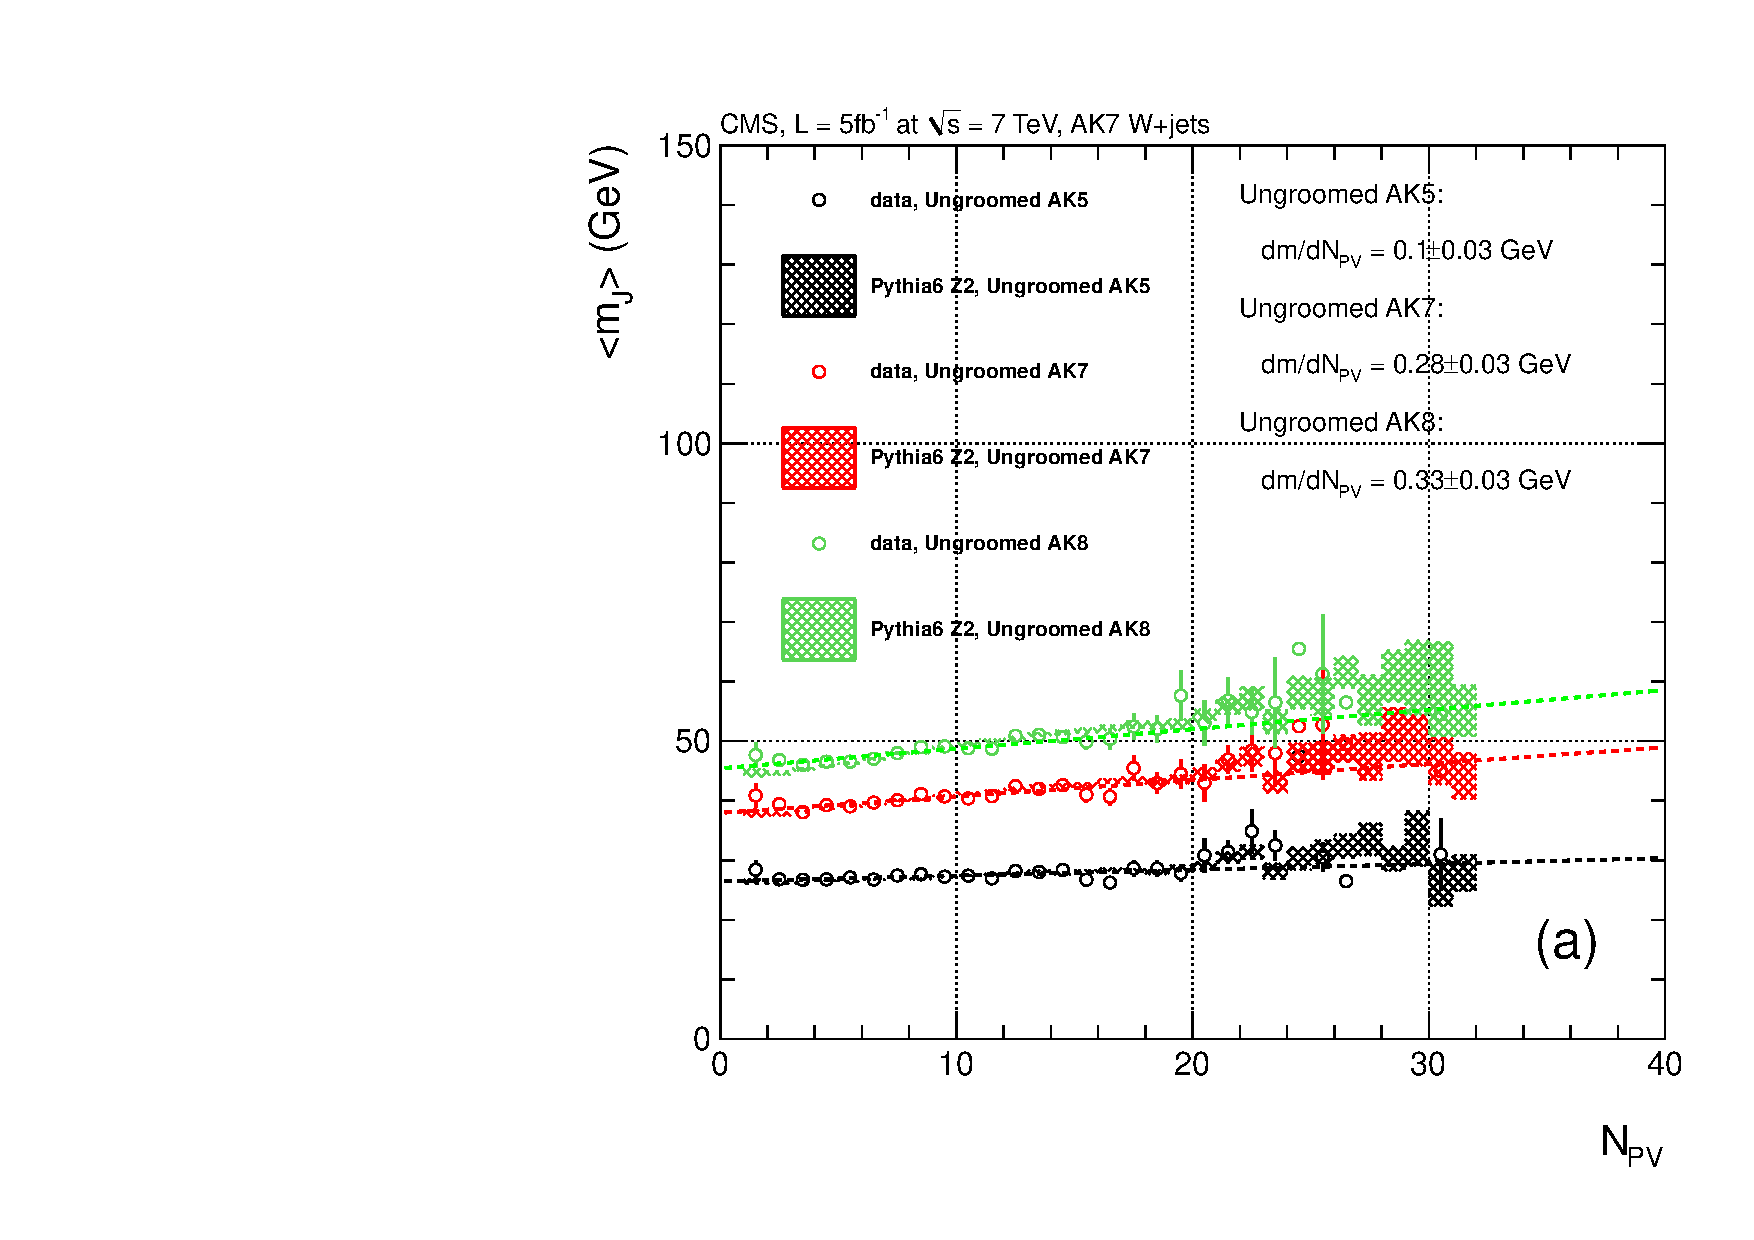
\includegraphics[width=0.495\textwidth]{figs/jetmassproj_vNV_set2.pdf}
%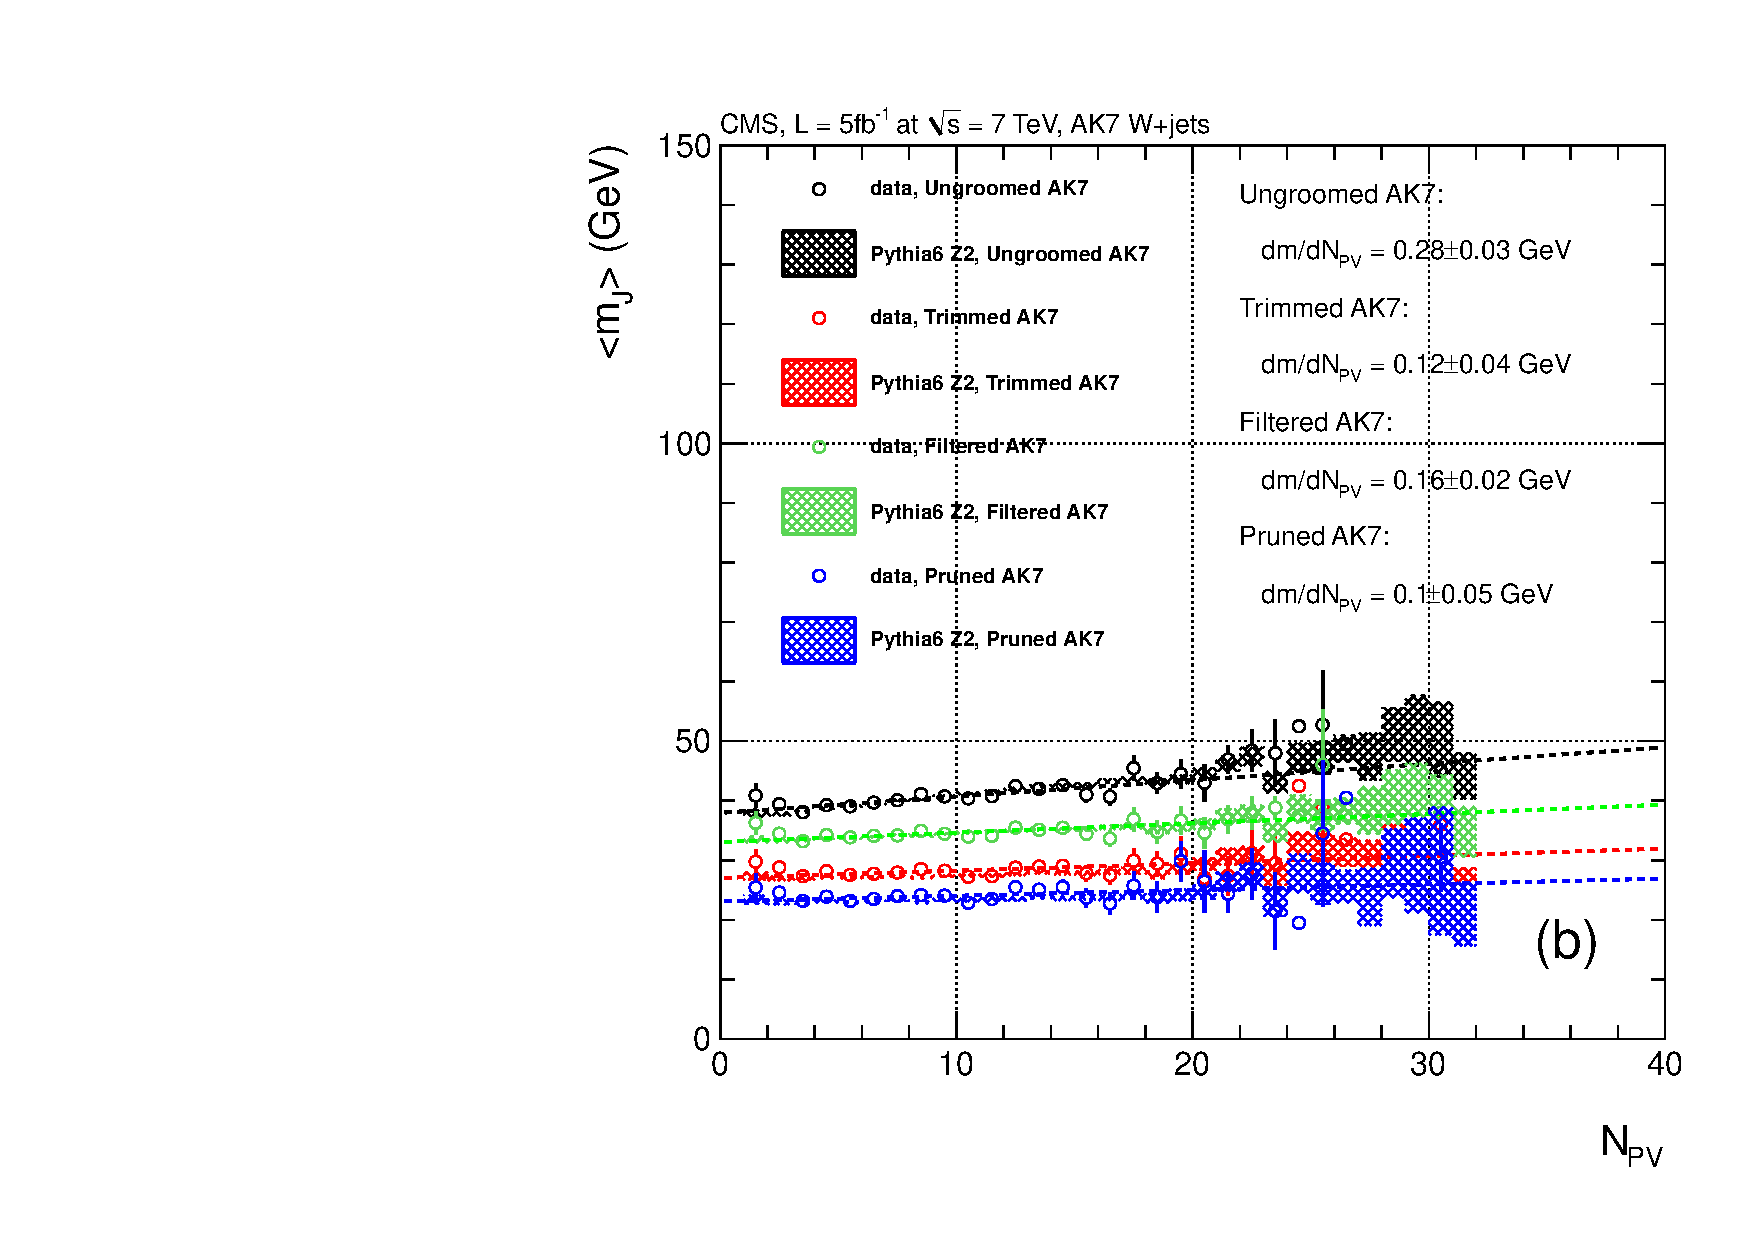
\includegraphics[width=0.495\textwidth]{figs/jetmassproj_vNV_set1.pdf}
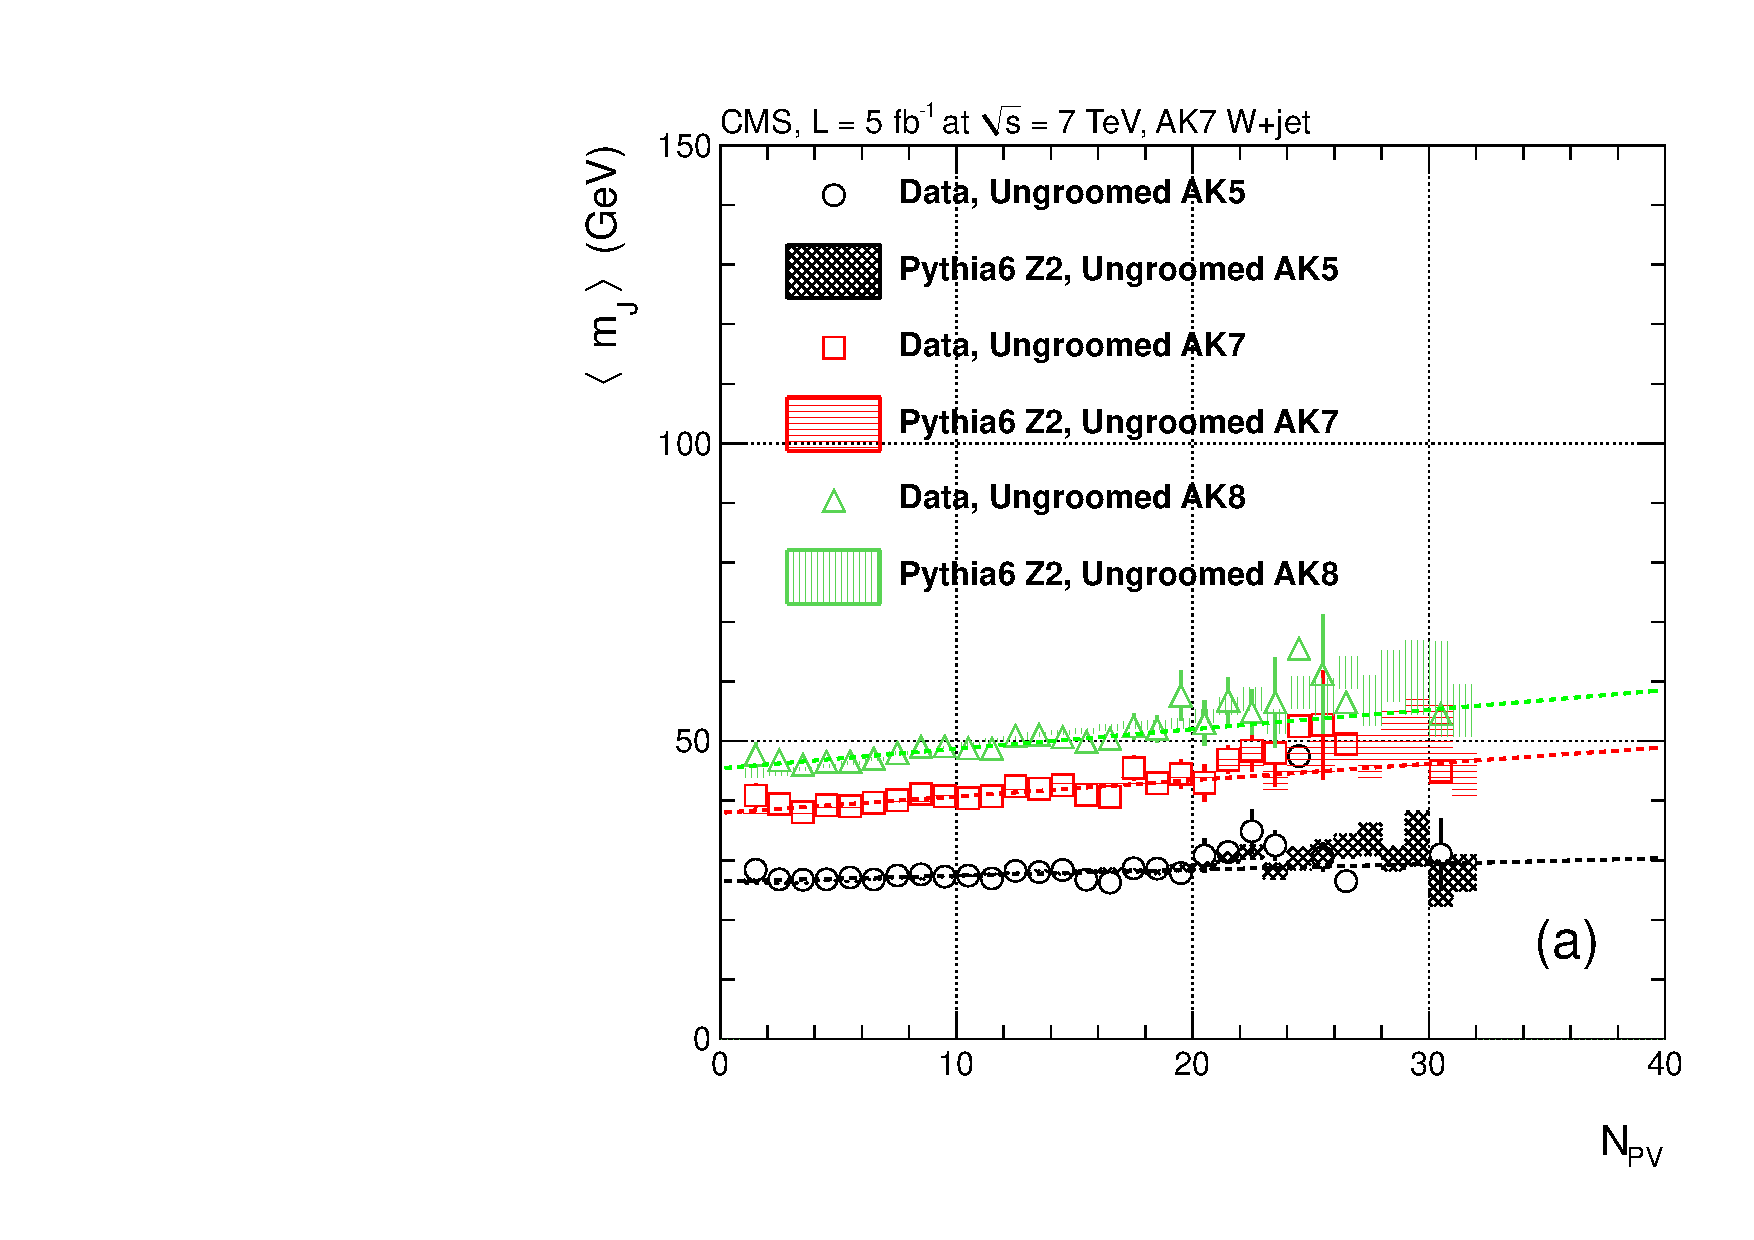
\includegraphics[width=0.495\textwidth]{figs/jetmassproj_vNV_set2_Wmunu.pdf}
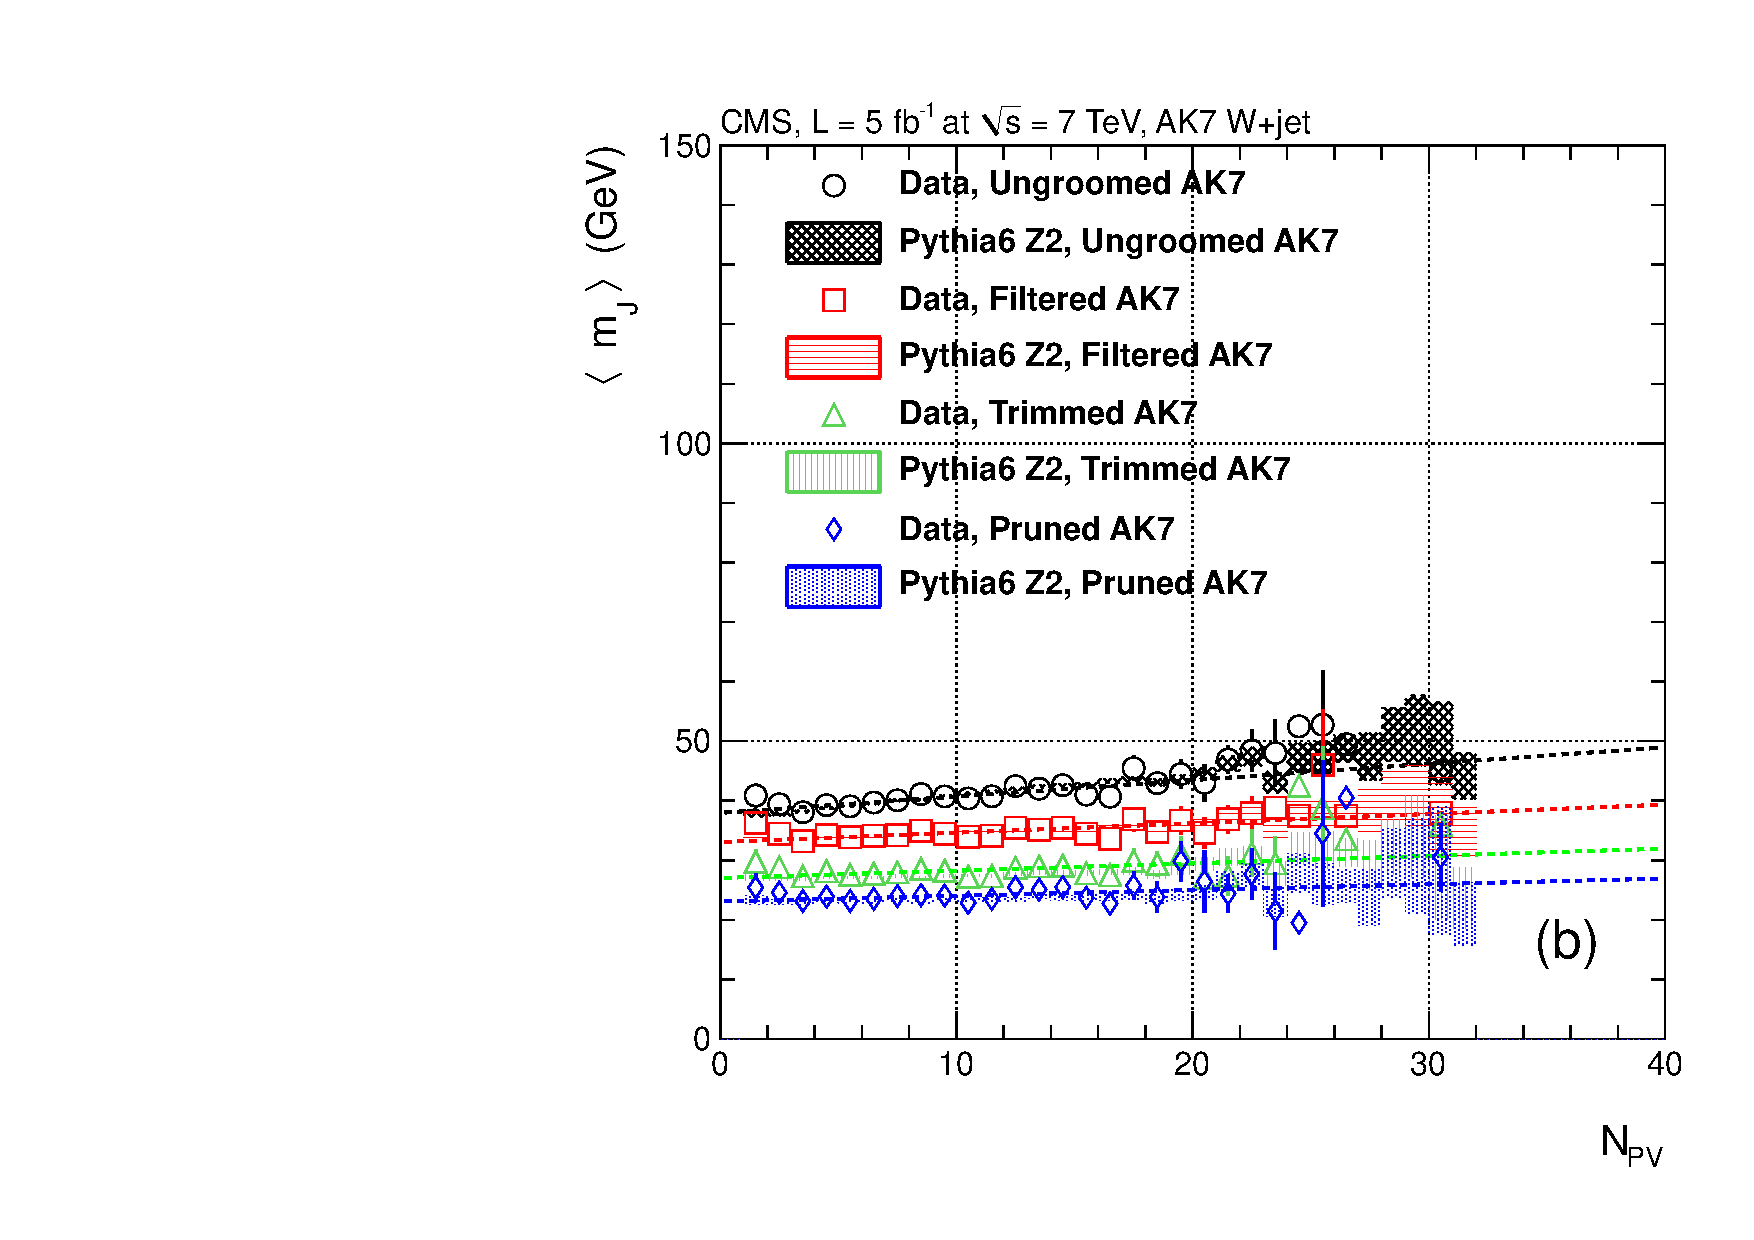
\includegraphics[width=0.495\textwidth]{figs/jetmassproj_vNV_set1_Wmunu.pdf}

\caption{Distributions of the average jet mass for AK jets as a function of the number of reconstructed primary vertices: (a) for different jet radii, and (b) for AK7 jets, comparing the impact of grooming algorithms to results without grooming.
\label{figs:histAK7MjetVsNvtx_nvtxPlots}}
\end{figure}


\begin{table}[!h]
\caption{Values of slopes for the dependence of $\langle m_J \rangle$ on $N_{\mathrm{PV}}$ for AK jets with different radii and clustering algorithms.}
\label{tab:slopes2}
\begin{center}
\begin{tabular}{ccc} \hline\hline
Jet R & Clustering Algorithm & $s_R$ (GeV/PV) \\ \hline
AK5 & ungroomed & $0.10 \pm 0.03$ (stat)   \\
AK7 & ungroomed & $0.28 \pm 0.03$ (stat)  \\
AK7 & filtered & $0.16 \pm 0.02$ (stat)  \\
AK7 & trimmed & $0.12 \pm 0.04$ (stat)  \\
AK7 & pruned  & $0.10 \pm 0.05$ (stat)  \\
AK8 & ungroomed & $0.33 \pm 0.03$ (stat)  \\
\hline\hline
\end{tabular}
\end{center}
\end{table}


%\begin{figure}[htbp]
%\centering
%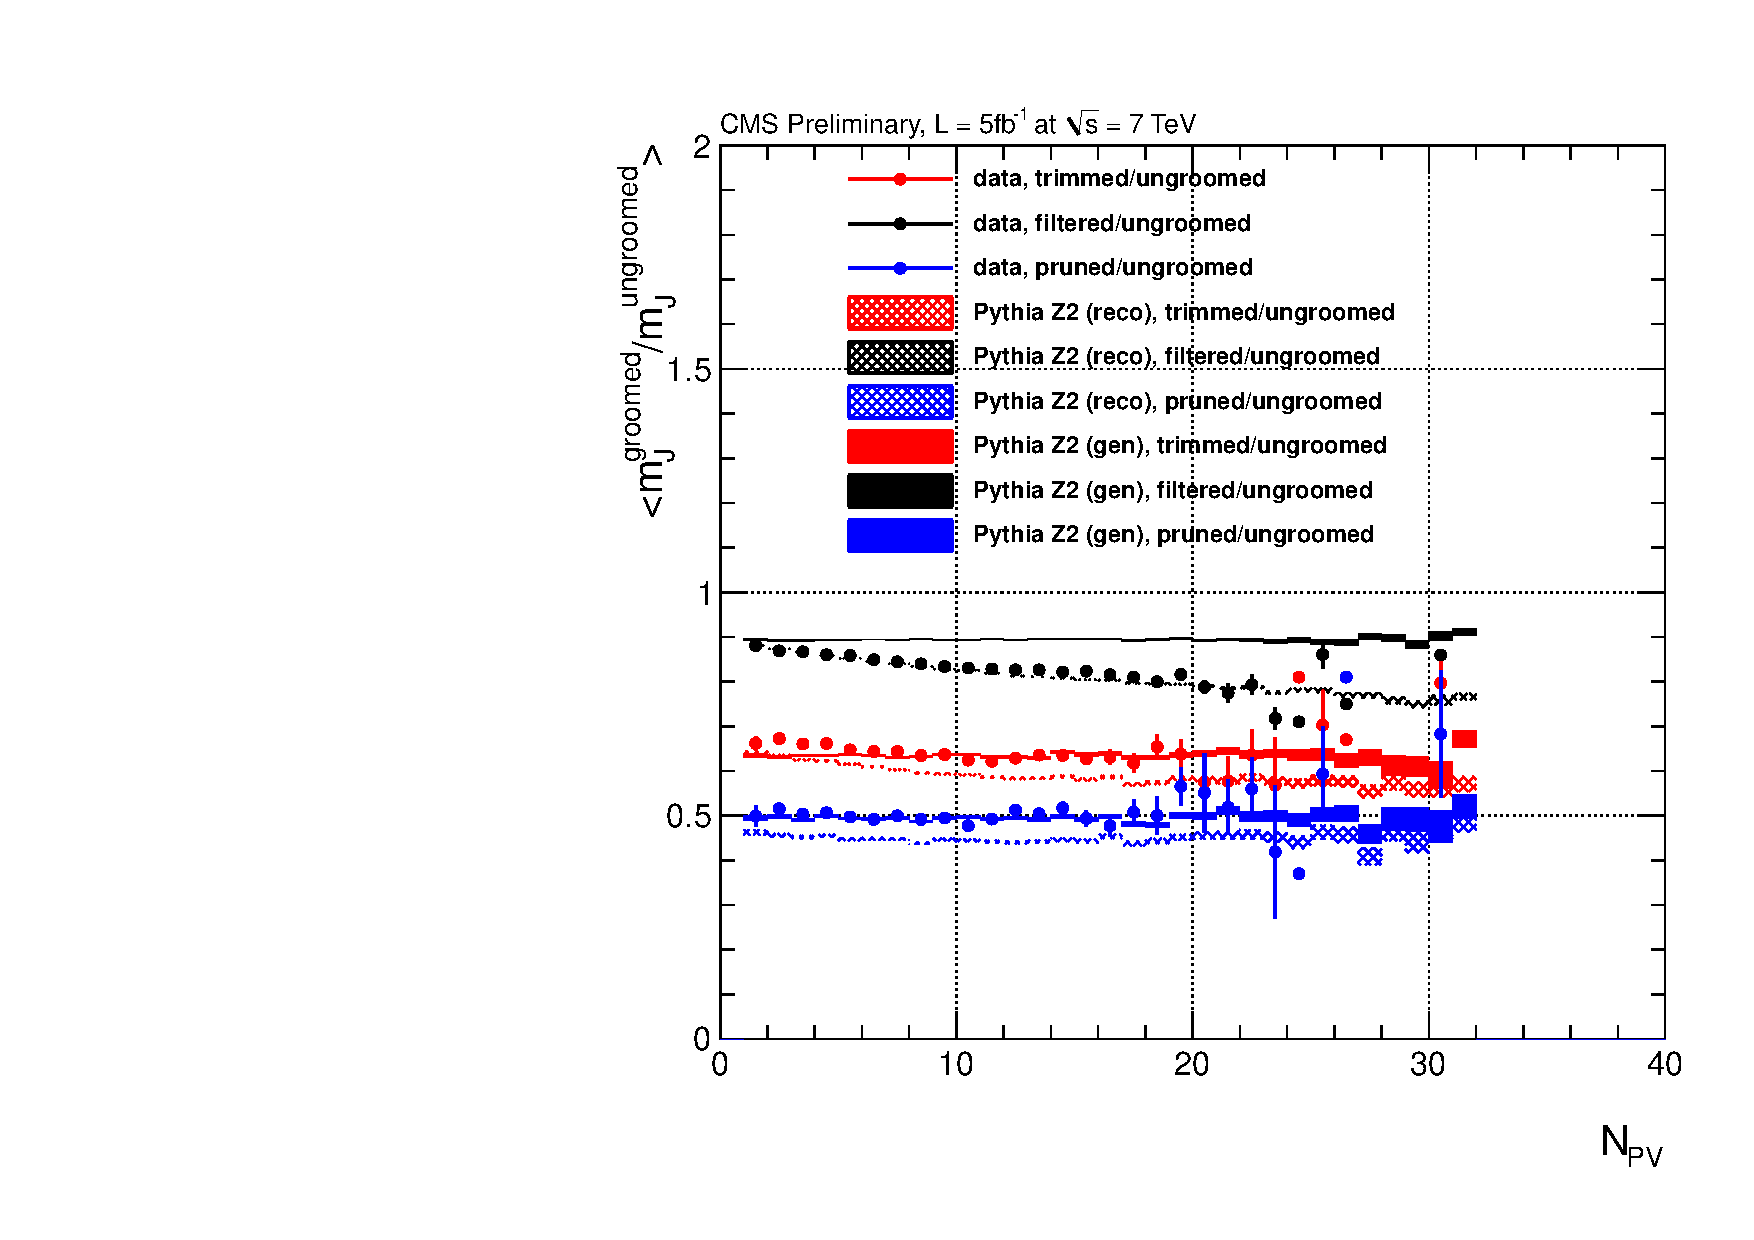
\includegraphics[width=0.495\textwidth]{figs/jetmass_ratioprofileNV_ak7.pdf}

%\caption{Detector-level distributions of the average jet mass for groomed AK jets divided by the jet mass of ungroomed jets 
%as a function of the number of reconstructed primary vertices. 
%\label{figs:histAK7MjetVsNvtx_nvtxPlots2}}
%\end{figure}



%The excellent data-MC agreement in these distributions as well as the reduced dependence on PU for the groomed met mass proves that the PU dependence of the grooming algorithms is well understood and that they are effective toward PU suppression.

The observed agreement between data and simulation in 
Fig.~\ref{figs:histAK7MjetVsNvtx_nvtxPlots} provides 
support for our characterization of jet grooming and pileup, and 
the decrease in slopes suggests
that grooming is indeed an effective tool for suppressing the impact
of pileup on jets with large $R$ parameters. 
